\documentclass[12pt,a4paper]{article}
\usepackage[utf8]{inputenc}
\usepackage{amsmath}
\usepackage{amsfonts}
\usepackage{amssymb}
\usepackage{enumerate}
\usepackage[spanish]{babel}
\usepackage{graphicx}
\usepackage{float}
\graphicspath{ {IMAGES/} }
\pagestyle{headings}
\author{Juan Sebastian Gonzalez Camacho (1968220), Andrés Felipe Ruíz Buriticá (1968171), Jhoan Sebastian Rojas Holguin (1958337), Carlos Alberto Delgado Galeano (1968127), Jesus Alberto Gil Ayala (1968231)}
\title{Borvo MO - Requirements Specification}
\begin{document}
\begin{titlepage}
\centering
{
\includegraphics[width=0.18 \textwidth]{logo.png} \par}
\vfill
{\bfseries\LARGE Universidad del Valle\par}
{\Large Sede Tuluá\par}
\vfill
{\scshape\Large Ingeniería de Sistemas \par}
\vfill
{\scshape\Huge Borvo - Medicinae Operam \par}
\vfill
{\itshape\Large Proyecto Final de Bases de Datos y Desarrollo de Software I \par}
\vfill
{\Large Autores: \par}
{\Large Juan Sebastian González Camacho - 1968220 \par}
{\Large Andrés Felipe Ruíz Buriticá - 1968171 \par}
{\Large Jhoan Sebastian Rojas Holguin - 1958337 \par}
{\Large Carlos Alberto Delgado Galeano - 1968127 \par}
{\Large Jesús Alberto Gil Ayala - 1968231 \par}
\vfill
{\Large 9 de Octubre del 2022 \par}
\end{titlepage}
\tableofcontents
\newpage
\section{Introducción}
Esta es la Especificación de Requisitos de Software para \emph{Borvo-Medicinae Operam}, un producto de software encargado de la gestión de información de la EPS ``Esperar para Salvarse''. Este documento ha sido elaborado a partir del estándar \textit{IEEE 830}.
\subsection{Propósito}
Definir y presentar de forma ordenada los requisitos y especificaciones que deberá cumplir el software \emph{Borvo-Medicinae Operam}, que elaboraremos para la EPS ``Esperar para Salvarse'', el cual permitirá gestionar la información de cotizantes, beneficiarios e instituciones externas asociadas a ella.
\subsection{Ámbitos del Sistema}
Con \emph{Borvo-Medicinae Operam} buscamos desarrollar un software web que sirva para mejorar los procesos y subprocesos de la EPS, con tal de fortalecer la gestión de la información de sus cotizantes, beneficiarios y las IPS asociadas para brindar un servicio oportuno.\\

Los usuarios tienen diferentes funciones según su rol: los administradores podrán gestionar afiliados, empresas, IPS, contratos, órdenes de servicio y generar reporte de afiliados por estado, órdenes por paciente y afiliados por empresa, los trabajadores pueden consultar su propia información y el banco puede cargar la información de los pagos que reportan las empresas, los cuales pueden hacerse individualmente o cargarse en bloque desde archivos.
\subsection{Definiciones, Acrónimos y Abreviaturas}
\begin{itemize}
\item \textbf{EPS:} Entidad Promotora de Salud.
\item \textbf{IPS:} Institución Prestadora de Salud.
\item \textbf{GUI:} Interfaz Gráfica de Usuario.
\item \textbf{IDE:} Entorno Integrado de Desarrollo.
\item \textbf{SGBD} Sistema de Gestión de Bases de Datos.
\item \textbf{HTML:} Lenguaje de Marcas de Hipertexto.
\item \textbf{MER:} Modelo Entidad - Relación.
\item \textbf{UML:} Lenguaje Unificado de Modelado.
\item \textbf{Software:} Conjunto de programas y rutinas que permiten a la computadora realizar determinadas tareas.
\item \textbf{Front-end:} Es la parte de una aplicación que interactúa con los usuarios, es conocida como el lado del cliente. Básicamente es todo lo que vemos en la pantalla cuando accedemos a un sitio web o aplicación: tipos de letra, colores, adaptación para distintas pantallas, los efectos del ratón, teclado, movimientos, desplazamientos, efectos visuales… y otros elementos que permiten navegar dentro de una página web. Este conjunto crea la experiencia del usuario.
\item \textbf{Back-end:} Es la parte del desarrollo web que se encarga de que toda la lógica de una página web  funcione. Se trata del conjunto de acciones que pasan en una web pero que no vemos como, por ejemplo, la comunicación con el servidor.
\item \textbf{JavaScript:} Es un lenguaje de programación interpretado, dialecto del estándar ECMAScript. Se define como orientado a objetos, basado en prototipos, imperativo, débilmente tipado y dimámico.
\item Aquí se van agregando otras abreviaturas, acrónimos y definiciones.
\end{itemize}
\subsection{Equipo de Desarrollo de Software}
Nuestra empresa desarrolladora, Memento Coding, es una idea que nació de un grupo de estudiantes de Ingeniería de Sistemas de la Universidad del Valle apasionados por el desarrollo de aplicaciones web:

\begin{itemize}
\item Juan Sebastian Gonzalez Camacho (1968220)
\item Andrés Felipe Ruíz Buriticá (1968171)
\item Jhoan Sebastian Rojas Holguin (1958337)
\item Carlos Alberto Delgado Galeano (1968127)
\item Jesus Alberto Gil Ayala (1968231)
\end{itemize}
\begin{figure}[H]
\centering
{
\includegraphics[width=0.5 \textwidth]{logo_memento} \par}
\caption{Logo de nuestra empresa Memento Coding}
\end{figure}
\subsection{Referencias}
\begin{itemize}
\item Especificación de Requisitos según el estándar de IEEE 830.
\end{itemize}
\subsection{Visión General del Documento}
Este documento contiene la descripción del software, sus requerimientos funcionales y no funcionales, casos de uso y escenarios, el diseño de la interfaz, la arquitectura, el modelo de la base de datos y la implementación.
\section{Descripción General}
La aplicación web \emph{Borvo-Medicinae Operam} es un software integrado que maneja la información y las actividades de la Entidad Promotora de Salud de forma digital para una administración más eficaz, con mejor rendimiento y mayor confiabilidad. A partir de tecnologías de vanguardia que implementan interfaces claras e intuitivas, se facilita la gestión de los detalles del paciente, la información administrativa, médica y financiera del centro de salud.
\subsection{Perspectiva del Producto}
\emph{Borvo-Medicinae Operam} está planeado como un software independiente, que no requiere sistemas externos para su funcionamiento e interacción. 
\subsection{Funciones del Producto}
\vspace{5mm}
\begin{figure}[H]
\centering
{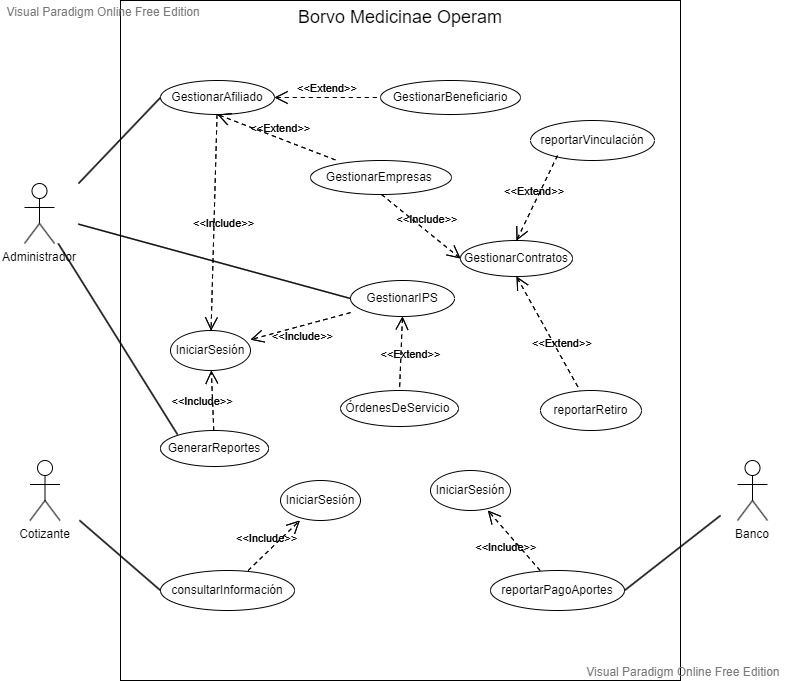
\includegraphics[width=1 \textwidth]{use_cases_diagram.png} \par}
\caption{Diagrama de Casos de Uso.}
\end{figure}
\subsection{Características de los Usuarios}
\begin{center}
\begin{tabular}{|p{3.5cm}| p{11.5cm}|}
\hline 
\multicolumn{2}{|c|}{\textbf{Administrador}} \\ 
\hline 
\textbf{Nivel Educativo} & Educación superior / Especialista en TICs.\\ 
\hline 
\textbf{Experiencia} & Manejo de TICs y gestión de sistemas de información. \\ 
\hline 
\textbf{Actividades} & Gestionar afiliados, empresas IPS, contratos, órdenes de servicio y generar reporte de afiliados por estado, órdenes por paciente y afiliados por empresa. \\ 
\hline 
\end{tabular}
\vspace{5mm}

\begin{tabular}{|p{3.5cm}| p{11.5cm}|}
\hline 
\multicolumn{2}{|c|}{\textbf{Trabajador}} \\ 
\hline 
\textbf{Nivel Educativo} & Educación secundaria.\\ 
\hline 
\textbf{Experiencia} & Manejo de TICs.\\ 
\hline 
\textbf{Actividades} & Consultar su propia información.\\ 
\hline 
\end{tabular}
\vspace{5mm}

\begin{tabular}{|p{3.5cm}| p{11.5cm}|}
\hline 
\multicolumn{2}{|c|}{\textbf{Banco}} \\ 
\hline 
\textbf{Nivel Educativo} & Educación superior / Especialista en TICs.\\ 
\hline 
\textbf{Experiencia} & Gestión de sistemas de información.\\ 
\hline 
\textbf{Actividades} & Puede cargar la información de los pagos que reportan las empresas, los cuales pueden hacerse individualmente o cargarse en bloque desde archivos.\\ 
\hline 
\end{tabular}
\vspace{5mm}
\end{center}
\subsection{Restricciones}
\begin{itemize}
\item El software requiere conexión a internet para su funcionamiento.
\item El software debe contar con un sistema de login de sesión.
\item Todo usuario Administrador debe tener noción de la gestión de la EPS.
\item El software debe funcionar las 24 horas del día, los 7 días de la semana.
\item El software debe ser accesible desde cualquier dispositivo.
\item Aquí se van añadiendo restricciones a medida que se va desarrollando el software (p.ej uso de algun framework en especifico, de alguna API, tipo de aplicación, etc).
\end{itemize}
\subsection{Suposiciones y Dependencias}
\begin{itemize}
\item Los equipos en donde se utilice el software deben contar con un mínimo de recursos, navegador y una buena conexión a Internet.
\end{itemize}
\subsection{Requisitos Futuros}
\section{Requisitos Específicos}
\subsection{Interfaces Externas}
\subsection{Funciones}
\begin{center}
\begin{tabular}{|p{5.5cm}| p{9.5cm}|}
\hline 
\multicolumn{2}{|c|}{\textbf{CU\#1 - GestionarIPS}} \\ 
\hline 
\textbf{Descripción} & Permite registrar una IPS dentro del sistema. \\ 
\hline 
\textbf{Actores} & Es iniciado por Administrador. \\ 
\hline 
\textbf{Pre-condición} & El administrador debe haberse autenticado de forma exitosa en el sistema de acuerdo a su perfil. \\ 
\hline 
\textbf{Flujo de Eventos} & Flujo Principal (P):

\textbf{P1.} El administrador selecciona la opción de Registrar nueva IPS.

\textbf{P2.} El sistema despliega un formulario para registrar la IPS.

\textbf{P3.} El administrador ingresa el NIT, razón social, nivel de atención y servicios que presta la IPS.

\textbf{P4.} El administrador da clic en el botón Guardar para enviar el formulario.

\textbf{P5.} El sistema valida los datos (A1).

\textbf{P6.} El sistema muestra el mensaje de confirmación.
\\
\hline 
\textbf{Flujo Alterno} &  Flujo Alterno (A):

\textbf{A1.} La IPS ya está registrada.

	En P5:
	
	5.1. Si el NIT corresponde a una IPS ya registrada, el sistema debe mostrar un mensaje indicando esto.
	
	5.2. Si es error de digitación, retorna a P2 para ingresar nuevamente los dato sen el formulario. \\ 
\hline 
\textbf{Post-condición}  & Registro exitoso de la IPS dentro del sistema. \\ 
\hline 
\textbf{Requisitos No Funcionales} & Ninguno \\ 
\hline 
\end{tabular}
\vspace{5mm}

\begin{tabular}{|p{5.5cm}| p{9.5cm}|}
\hline 
\multicolumn{2}{|c|}{\textbf{CU\#2 - ReportarPagoAportes}} \\ 
\hline 
\textbf{Descripción} & Permite reportar dentro del sistema el pago de aportes que hace cada cotizante. \\ 
\hline 
\textbf{Actores} & Es iniciado por Banco. \\ 
\hline 
\textbf{Pre-condición} & El banco debe haberse autenticado de forma exitosa en el sistema de acuerdo a su perfil. \\ 
\hline 
\textbf{Flujo de Eventos} & Flujo Principal (P):

\textbf{P1.} El banco selecciona la opción de Reporte pago de aportes.

\textbf{P2.} El sistema despliega un formulario para hacer el reporte del pago.

\textbf{P3.} El banco ingresa la fecha de pago, el valor pagado, la información del cotizante y la información de la empresa que hace el pago (si el cotizante es dependiente).

\textbf{P4.} El banco da clic en el botón Guardar para enviar el formulario.

\textbf{P5.} El sistema valida los datos (A1).

\textbf{P6.} El sistema muestra un mensaje de confirmación.
\\
\hline 
\textbf{Flujo Alterno} &  Flujo Alterno (A):

\textbf{A1.} El pago de aportes ya se ha realizado.

	En P5:
	
	5.1. Si no hay un pago de aportes pendiente, el sistema debe mostrar un mensaje indicando esto.
	
	5.2. Si es error de digitación, retorna a P2 para ingresar nuevamente los dato sen el formulario. \\ 
\hline 
\textbf{Post-condición}  & Reporte de pago de aportes realizados durante el mes. \\ 
\hline 
\textbf{Requisitos No Funcionales} & Ninguno \\ 
\hline 
\end{tabular}
\vspace{5mm}

\begin{tabular}{|p{5.5cm}| p{9.5cm}|}
\hline 
\multicolumn{2}{|c|}{\textbf{CU\#3 - ConsultarInformacionPropia}} \\ 
\hline 
\textbf{Descripción} & Permite consultar la información del cotizante actualmente autenticado. \\ 
\hline 
\textbf{Actores} & Es iniciado por Cotizante. \\ 
\hline 
\textbf{Pre-condición} & El cotizante debe haberse autenticado de forma exitosa en el sistema de acuerdo a su perfil. \\ 
\hline 
\textbf{Flujo de Eventos} & Flujo Principal (P):

\textbf{P1.} El cotizante selecciona la opción de Ver Perfil.

\textbf{P2.} El sistema despliega una página con la información del cotizante y sus beneficiarios (si los tiene).
\\
\hline 
\textbf{Flujo Alterno} &  Flujo Alterno (A):
\\ 
\hline 
\textbf{Post-condición}  & El cotizante consulta su propia información que está guardada en el sistema. \\ 
\hline 
\textbf{Requisitos No Funcionales} & Ninguno \\ 
\hline 
\end{tabular}
\vspace{5mm}

\begin{tabular}{|p{5.5cm}| p{9.5cm}|}
\hline 
\multicolumn{2}{|c|}{\textbf{CU\#4 - IniciarSesión}} \\ 
\hline 
\textbf{Descripción} & Permite al usuario ingresar al sistema según su rol. \\ 
\hline 
\textbf{Actores} & Es iniciado por Administrador, Cotizante o Banco. \\ 
\hline 
\textbf{Pre-condición} & El usuario debe estar previamente registrado en el sistema. \\ 
\hline 
\textbf{Flujo de Eventos} & Flujo Principal (P):

\textbf{P1.} El usuario solicita al sistema entrar en la aplicación.

\textbf{P2.} El sistema despliega un login en el que solicita al usuario introducir su usuario y contraseña.

\textbf{P3.} El usuario da clic en ingresar.

\textbf{P4.} El sistema comprueba los datos introducidos.

\textbf{P5.} Si los datos son correctos, el sistema ingresa a la página de inicio para el rol del usuario que ingresó.
\\
\hline 
\textbf{Flujo Alterno} &  Flujo Alterno (A):

\textbf{A1.} El nombre de usuario o contraseña son incorrectos.

	En P4:
	
	4.1. Si el usuario es incorrecto, el sistema muestra un mensaje indicando que el usuario es incorrecto y retorna a P2.
	
	4.2. Si la contraseña es incorrecta, el sistema muestra un mensaje indicando que la contraseña es incorrecta y retorna a P2. \\ 
\hline 
\textbf{Post-condición}  & El usuario ingresa al sistema. \\ 
\hline 
\textbf{Requisitos No Funcionales} & Ninguno \\ 
\hline 
\end{tabular}
\vspace{5mm}

\begin{tabular}{|p{5.5cm}| p{9.5cm}|}
\hline 
\multicolumn{2}{|c|}{\textbf{CU\#5 - GestionarBeneficiario}} \\ 
\hline 
\textbf{Descripción} & Permite registrar la información de las personas que son beneficiarios de los afiliados titulares. \\ 
\hline 
\textbf{Actores} & Es iniciado por Administrador. \\ 
\hline 
\textbf{Pre-condición} & El administrador debe haberse autenticado de forma exitosa en el sistema de acuerdo a su perfil. \\ 
\hline 
\textbf{Flujo de Eventos} & Flujo Principal (P):

\textbf{P1.} El administrador debe seleccionar la opción Gestionar beneficiario en el sistema.

\textbf{P2.} El sistema despliega un formulario para registrar los datos de los beneficiarios.

\textbf{P3.} El administrador registra DNI, Nombres, Apellidos, Fecha de Nacimiento, Ciudad de Residencia, Teléfono, e-mail, Dirección, Género, Estado Civil, Estado Actual, Parentesco con el cotizante.

\textbf{P4.} El administrador da clic en el botón Guardar para enviar el formulario.

\textbf{P5.} El sistema valida los datos (A1).

\textbf{P6.} El sistema muestra el mensaje de confirmación.
\\
\hline 
\textbf{Flujo Alterno} &  Flujo Alterno (A):

\textbf{A1.} El beneficiario ya se encontraba registrado.

	En P4:
	
	4.1. Si el DNI corresponde a un beneficiario ya registrado, el sistema debe mostrar un mensaje indicando esto.
	
	4.2. Si es error de digitación, retorna a P2 para ingresar nuevamente los datos en el formulario. \\ 
\hline 
\textbf{Post-condición}  & El beneficiario queda registrado en el sistema. \\ 
\hline 
\textbf{Requisitos No Funcionales} & Ninguno \\ 
\hline 
\end{tabular}
\vspace{5mm}

\begin{tabular}{|p{5.5cm}| p{9.5cm}|}
\hline 
\multicolumn{2}{|c|}{\textbf{CU\#6 - GestionarAfiliado}} \\ 
\hline 
\textbf{Descripción} & Permite registrar la información de las personas que los afiliados. \\ 
\hline 
\textbf{Actores} & Es iniciado por Administrador. \\ 
\hline 
\textbf{Pre-condición} & El administrador debe haberse autenticado de forma exitosa en el sistema de acuerdo a su perfil. \\ 
\hline 
\textbf{Flujo de Eventos} & Flujo Principal (P):

\textbf{P1.} El administrador debe seleccionar la opción Gestionar afiliado en el sistema.

\textbf{P2.} El sistema despliega un formulario para registrar los datos de los afiliados.

\textbf{P3.} El administrador registra DNI, Nombres, Apellidos, Fecha de Nacimiento, Ciudad de Residencia, Teléfono, e-mail, Dirección, Género, Estado Civil, Estado Actual, Fecha de Primera Afiliación, Salario, Rango Salarial.

\textbf{P4.} El administrador da clic en el botón Guardar para enviar el formulario.

\textbf{P5.} El sistema valida los datos (A1).

\textbf{P6.} El sistema muestra el mensaje de confirmación.
\\
\hline 
\textbf{Flujo Alterno} &  Flujo Alterno (A):

\textbf{A1.} El afiliado ya se encontraba registrado.

	En P4:
	
	4.1. Si el DNI corresponde a un afiliado ya registrado, el sistema debe mostrar un mensaje indicando esto.
	
	4.2. Si es error de digitación, retorna a P2 para ingresar nuevamente los datos en el formulario. \\ 
\hline 
\textbf{Post-condición}  & El afiliado queda registrado en el sistema. \\ 
\hline 
\textbf{Requisitos No Funcionales} & Ninguno \\ 
\hline 
\end{tabular}
\vspace{5mm}

\begin{tabular}{|p{5.5cm}| p{9.5cm}|}
\hline 
\multicolumn{2}{|c|}{\textbf{CU\#7 - GestionarEmpresa}} \\ 
\hline 
\textbf{Descripción} & Permite registrar la información de las empresas a las que pertenecen los afiliados. \\ 
\hline 
\textbf{Actores} & Es iniciado por Administrador. \\ 
\hline 
\textbf{Pre-condición} & El administrador debe haberse autenticado de forma exitosa en el sistema de acuerdo a su perfil. \\ 
\hline 
\textbf{Flujo de Eventos} & Flujo Principal (P):

\textbf{P1.} El administrador debe seleccionar la opción Gestionar empresa en el sistema.

\textbf{P2.} El sistema despliega un formulario para registrar los datos de las empresas.

\textbf{P3.} El administrador registra NIT, Ciudad, Teléfono, Razón social, Nombre del contacto.

\textbf{P4.} El administrador da clic en el botón Guardar para enviar el formulario.

\textbf{P5.} El sistema valida los datos (A1).

\textbf{P6.} El sistema muestra el mensaje de confirmación.
\\
\hline 
\textbf{Flujo Alterno} &  Flujo Alterno (A):

\textbf{A1.} La empresa ya se encontraba registrada.

	En P4:
	
	4.1. Si el NIT corresponde a una empresa ya registrada, el sistema debe mostrar un mensaje indicando esto.
	
	4.2. Si es error de digitación, retorna a P2 para ingresar nuevamente los datos en el formulario. \\ 
\hline 
\textbf{Post-condición}  & La empresa queda registrada en el sistema. \\ 
\hline 
\textbf{Requisitos No Funcionales} & Ninguno \\ 
\hline 
\end{tabular}
\end{center}
\subsection{Requisitos de Rendimiento}
Ninguno
\subsection{Restricciones de Diseño}
\begin{figure}[H]
\centering
{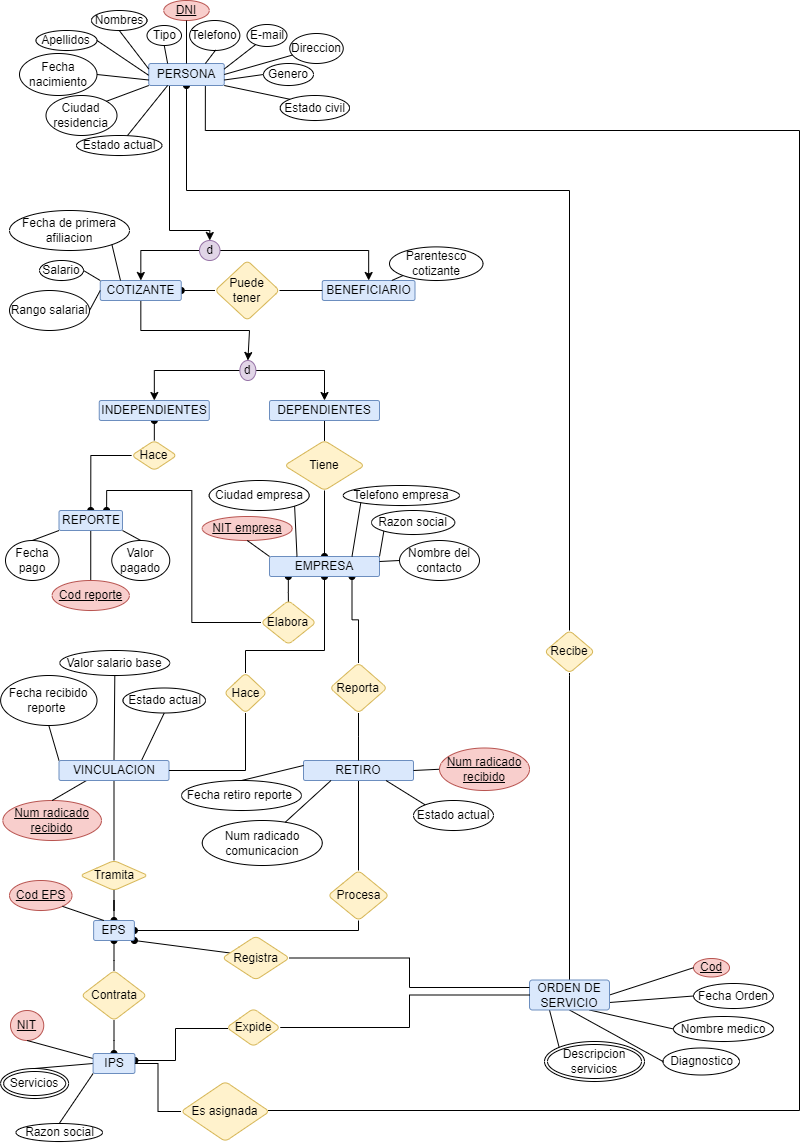
\includegraphics[width=1 \textwidth]{entity_relationship_model.png} \par}
\caption{Modelo Entidad - Relación.}
\end{figure}
\subsection{Atributos del Sistema}
Ninguno
\subsection{Otros Requisitos}
Ninguno
\section{Apéndices}
Nothing
\end{document}
